\chapter{Zufallsvariablen (ZV)}
Laut Oli sehr wichtig!\medskip\\
\textbf{Definition}:\\
Eine ZV ist eine Funktion X:$\Omega$ $\rightarrow \mathbb{R}$\smallskip\\\textbf{Beispiel}:\\
2 Würfel. \hspace{1cm}$\Omega = \{(a_1,a_2): a_1,a_2 \in \{1,...,6\}\}$\medskip\\
Erste Augenzahl: $X_1(a_1,a_2)=a_1$\\
Zweite Augenzahl $X_2(a_1,a_2)=a_2$\\
Augensumme: $X(a_1,a_2) = a_1 + a_2 \qquad x = x_1 + x_2$\\
Größe Augenzahl: $y(a_1,a_2)=max(a_1,a_2)$\medskip\\
\textbf{In dieser Vorlesung sei $\Omega$ immer endlich}\medskip\\
\textbf{Definition}:\\
Eine Verteilung einer ZV X ist die Angabe der Werte und der Wkeiten dieser Werte.\smallskip\\
\begin{tabbing}
	Zähldichte von X : $\Omega \rightarrow\mathbb{R}$ ist\= $P_x:\mathbb{R}\rightarrow[0,1]$\\\>
	$P_x(t)=\mathds{P}\underbrace{[x = t]}_\text{Er.} = \mathds{P}[\underbrace{\{w \in \Omega:X(\omega)=t\}}_{x^{-1}(t)}]$
\end{tabbing}
\textbf{Beispiel}: 2 Würfel. \hspace{1cm} $x(a_1,a_2) = a_1 + a_2$ Augensumme\\
\begin{tabular}{c|c|c|c|c|c|c|c|c|c|c|c|}
	t&2&3&4&5&6&7&8&9&10&11&12\\\hline
	$\mathds{P}[x=t]$&$\frac{1}{36}$&$\frac{2}{36}$&$\frac{3}{36}$&$\frac{4}{36}$&$\frac{5}{36}$&$\frac{6}{36}$&$\frac{5}{36}$&$\frac{4}{36}$&$\frac{3}{36}$&$\frac{2}{36}$&$\frac{1}{36}$
\end{tabular}\smallskip\\
\{x=2\} = \{(1,1)\}\\
\{x=3\}=\{(1,2),(2,1)\}\\
\{x=4\} = \{(1,3),(3,1),(2,2)\}\\
...\medskip\\
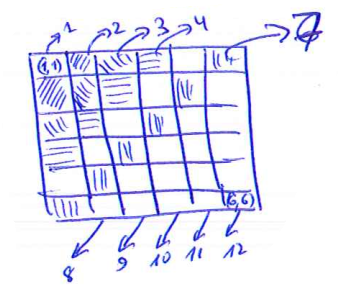
\includegraphics[width=0.4\textwidth]{img/okay.PNG}\\

\begin{math}
P_x(t)=
\begin{cases}
	\dfrac{t-1}{36}&, t \in \{2,...,7\}\medskip\\
	\dfrac{13-t}{36}& , t \in \{7,...,12\}\medskip\\
	0, t \notin \{2,...,12\}
\end{cases}
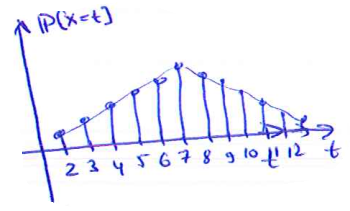
\includegraphics[width=0.4\textwidth]{img/diaa.PNG}
\end{math}\begin{floatingfigure}[r]{6cm}
	\mbox{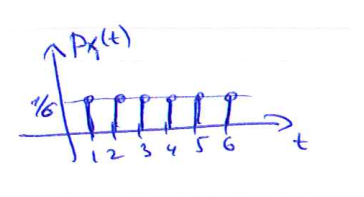
\includegraphics[width=0.4\textwidth]{img/dia.PNG}}
\end{floatingfigure}
Für die erste Augenzahl $x_1(a_1,a_2) = a_1$\medskip\\
\begin{tabular}{c|c|c|c|c|c|c}
	t&1&2&3&4&5&6\\\hline
	$\mathds{P[x_i = t]}$&$\frac{1}{6}$&$\frac{1}{6}$&$\frac{1}{6}$&$\frac{1}{6}$&$\frac{1}{6}$&$\frac{1}{6}$
\end{tabular}\medskip\\
\textbf{Eigenschaften der Zähldichte: }
\begin{enumerate}
	\item $P_x(t)\in [0,1]$
	\item $\sum_{t\in\mathbb{R}}P_x(t) = 1$
\end{enumerate}
\textbf{Beispiel}: Sei A $\subset$ $\Omega$\\
Indikatorvariable von A:\\
\begin{math}
\mathds{1}_A(\omega)=
\begin{cases}
1,& \omega \in A\\
0,& \omega \notin A
\end{cases}
\end{math}
\medskip\\
Grafik und Tabelle indikatorvariable\medskip\\
\textbf{Definition}: Sei X ZV mit Verteilung\medskip\\
\begin{tabular}{c|c|c|c|c}
	Werte&$y_1$&$y_2$&$y_3$&...\\\hline
	WKeiten&$P_1$&$P_2$&$P_3$&...
\end{tabular} \hspace{1cm}$\smallskip\\\mathds{P}[x = y_i] = p_i$\medskip\\
Erwartungswert von X ist $\mathds{E} X = \sum_i \underbrace{y_i}_\text{Werte} \underbrace{P_i}_\text{Wkeiten}$\medskip\\
\textbf{Beispiel}: 1 Würfel, $x_1$ Augenzahl\\
$\mathds{E}X_1 = 1*\frac{1}{6}+2*\frac{1}{6}+...+6*\frac{1}{6} = 3,5$\\
$\mathds{E}X$ ist \textbf{nicht} der wahrscheinlichste Wert: $\mathds{P} [X=3,5] = 0$\smallskip\\
\textbf{Bemerkung:}\\
Betrachte $n=10^6$ Würfe. Augenzahlen: $X_1,X_2,...,X_n$\\
Dann gilt $\dfrac{X_1+...+X_n}{n}\approx 3.5$\medskip\\
\textbf{Satz 9.1}$[\text{ alternative Formel für }\mathds{E}X]$\\
Sei $X:\Omega \rightarrow\mathbb{R}$. Dann gilt: 
$$\mathds{E}X = \sum_{\omega \in \Omega} X(\omega)\underbrace{\mathds{P}[\{\omega\}]}_{p(\omega)}$$
\textbf{Beweis}: Seien $y_1,...,y_m$ Werte von X\medskip\\
$A_1 = \{X = y_1\},\dots ,A_m=\{X=y_m\}$\\
$A_i = \{\omega \in \Omega:X(\omega)=y_i$s\}\smallskip\\
$\Omega = A_i \dot\cup A_2\dot\cup \dots\dot\cup A_m$ ist disj. Zerlegung\\
$\mathds{E}X \overset{\text{Def}}{=} \sum_i y_i*p_i = \sum_i y_i \mathds{P}[A_i]$\\
$\sum_iy_i\sum_{\omega \in A_i} p(\omega) \overset{w \in A_i}{=}\sum_i \sum_{\omega \in A_i} X(\omega)p(\omega)$ \\
$	\Rightarrow X(\omega)=y_i$\medskip\\
\textbf{Satz 9.2}. Seien $x,y :\Omega \rightarrow\mathbb{R}$ ZV\\
Dann gilt $\mathds{E}[x+y] = \mathds{E}X+\mathds{E}y$\medskip\\
\textbf{Beweis}: \\
$\mathds{E}[x+y] \underset{9.1}{=} \sum_{\omega \in \Omega}(x+y)(\omega)*p(\omega)=$\smallskip\\
$=\sum_{\omega \in \Omega} (X(\omega)+y(\omega))p(\omega) = \sum_{\omega \in \Omega}X(\omega)*p(\omega)+\sum_{\omega \in \Omega}y(\omega)*p(\omega)\overset{9.1}{=}\mathds{E}X+\mathds{E}y\qed$\medskip\\
\textbf{Bem.} Allgemein: Für ZV $X_1,\dots,X_n : \Omega \rightarrow \mathbb{R}:\mathds{E}[X_1+\dots+X_n] = \mathds{E}X_1+\dots+\mathds{E}X_n$\medskip\\
\textbf{Bem.} Sei $X:\Omega \rightarrow \mathbb{R}, a\in \mathbb{R}, \mathds{E}[a*X]=a*\mathds{E}X$\medskip\\
\textbf{Beispiel}: n Würfel. Augenzahlen: $X_1,\dots,X_n$ \hspace{1cm} Augensumme: S=$X_1+\dots+X_n$
$$\mathds{E}S=\mathds{E}X_n+\ldots+ \underbrace{\mathds{E}X_n}_{=3,5} = n*3,5$$
\textbf{Beispiel}: Lotto 6 aus 49. (ohne Zurücklegen) Tippe auf \{1,\dots,6\} \\
Sei S die Anzahl der richtig geratenen Zahlen.\medskip\\
Werte von S: 0,1,\dots,6\smallskip\\
$\mathds{P}[S=k] = \dfrac{\binom{6}{k}*\binom{43}{6-k}}{\binom{49}{6}} $ , für k $\in$ \{0,\ldots,6\}\medskip\\
\begin{math}
S = X_1+\dots+X_6, \text{wobei }\\
X_i = 
\begin{cases}
1,&\text{falls Ball \textbf{i} gezogen wurde}\\
0,&\text{sonst}
\end{cases}\smallskip\\
\mathds{E}S\underset{9.2}{=}\mathds{E}X_1+\dots+\mathds{E}X_6
\end{math}\medskip\\
\textbf{Bemerkung}: $\mathds{E1}_A=$\smallskip\\
\begin{tabular}{c|c}
	0&1\\\hline
	$1-\mathds{P}[A]$&$\mathds{P}[A]$
\end{tabular} =$\mathds{P}[A]$\medskip\\
\begin{math}
\mathds{E}X_i= \mathds{P}[\text{Ball \textbf{i} wurde gezogen}]\smallskip\\
= \dfrac{\binom{48}{5}}{\binom{49}{6}}\smallskip\\
=\dfrac{\left(\dfrac{48*47*46*45*44}{5!}\right)}{\left(\dfrac{48*47*46*45*44}{6!}\right)} = \dfrac{6!/5!}{49} = \dfrac{6}{49} \quad \forall i \in \{1,\dots,6\}\medskip\\
\mathds{E}S=\mathds{E}X_1+\dots\mathds{E}X_6=6*\dfrac{6}{49}=\dfrac{36}{49}
\end{math}\medskip\\
\textbf{Definition}:\\
Seien $X_1,\dots,X_n : \Omega \rightarrow\mathds{R}$ ZV\\
Sie heißen unabhängig, falls: 
$$\forall y_1,\dots,y_n \in \mathds{R}: \quad \mathds{P}[X_1 = y_1,X_2 =y_2,\dots,X_n=y_n]]$$
$$=\mathds{P}[X_1=y_1]*\dots*\mathds{P}[X_n]=y_n$$
\textbf{Bemerkung}: Sind $X_1,\dots,X_n$ unabg, dann gilt sogar:
$$\forall A_1,\dots,A_n \subset \mathds{R}: \mathds{P}[X_1 \in A_1,\dots,X_n \in A_n]$$
$$=\mathds{P}[X_1 \in A_1]*\dots*\mathds{P}[X_n \in A_n]$$\medskip\\
\textbf{Satz 9.3}:\\
Seien $X,Y :\Omega \rightarrow \mathds{R} $ \textbf{unabh}. ZV\\
Dann gilt $\mathds{E}[X*Y]= \mathds{E}X*\mathds{E}Y$\medskip\\
\textbf{2 Eigenschaften}:
\begin{enumerate}
	\item $\mathds{E}[x+y] = \mathds{E}x+\mathds{E}y \quad \forall x,y$
	\item $ \mathds{E}[x*y] = \mathds{E}x*\mathds{E}\text{$ y $ } \forall \text{unabh. } x,y$
\end{enumerate}